%%% File encoding: UTF-8
%% äöüÄÖÜß  <-- no German Umlauts here? Use an UTF-8 compatible editor!

%%% Magic comments for setting the correct parameters in compatible IDEs
% !TeX encoding = utf8
% !TeX program = pdflatex
% !TeX spellcheck = en
% !BIB program = biber

% FIXME is punctuation always BEHIND source?

\documentclass[master,english,smartquotes]{hgbthesis}
% Permissible options in [..]:
%   Type of work: diploma, master (default), bachelor, internship
%   Main language: german, english (default)
%		smartquotes: for simplified insertion of quotes (only "...")
%%%----------------------------------------------------------

\RequirePackage[utf8]{inputenc}		% Remove when using lualatex or xelatex entfernen!
\RequirePackage[version=4]{mhchem}
\RequirePackage{mol2chemfig}
\RequirePackage{chemfig}
\RequirePackage{multirow}
\RequirePackage{nicefrac}

%Make ((sub)sub)sections include their graphics without floating into next ((sub)sub)section.
\usepackage{placeins}
\let\Oldsection\section
\renewcommand{\section}{\FloatBarrier\Oldsection}
\let\Oldsubsection\subsection
\renewcommand{\subsection}{\FloatBarrier\Oldsubsection}
\let\Oldsubsubsection\subsubsection
\renewcommand{\subsubsection}{\FloatBarrier\Oldsubsubsection}

\graphicspath{{images/}}    % location of images and graphics
\logofile{logo.eps}	% logo file = images/logo.eps (use \logofile{} for no logo)
\bibliography{references}  	% name of bibliography file (references.bib)

%%%----------------------------------------------------------
% Title page entries
%%%----------------------------------------------------------

%%% Entries for ALL types of work: --------------------------
\title{Bistability and state switching in computational dynamic histone modification models}
\author{Michel Krecké}

%\programtype{Fachhochschul-Bachelorstudiengang}		% select/edit
\programtype{Master of Science}

\programname{Bioinformatik}
\placeofstudy{Leipzig}
\dateofsubmission{2021}{05}{10}	% {YYYY}{MM}{DD} % TODO: set to correct date

\advisor{Prof. Dr. Sonja Prohaska}	% optional
\secondAdvisor{Dr. Christian Arnold}

\hyphenation{nuc-leo-some}
\hyphenation{nuc-leo-somes}
\hyphenation{pre-dom-in-ant}

%\strictlicense		%%% restrictive license instead of Creative Commons (discouraged!)

%%%----------------------------------------------------------
\begin{document}
%%%----------------------------------------------------------

%%%----------------------------------------------------------
\frontmatter							% title part (roman page numbers)
%%%----------------------------------------------------------

\maketitle
\tableofcontents

% \chapter{Preface}




 	% preface is optional
% \chapter{Abstract}
Main question: How to establish bistability with EpiDynast?
	next neighbour not enough (how to prove?)
	how to find all the possibilities to establish bistability?
		(Mathematical) basis for bistability\\

This should be a 1-page (maximum) summary of your work in English.


% \chapter{Kurzfassung}

\begin{german}
An dieser Stelle steht eine Zusammenfassung der Arbeit, Umfang
max.\ 1 Seite. 
...
\end{german}

%%%----------------------------------------------------------
\mainmatter          			% main part (arabic page numbers)
%%%----------------------------------------------------------

\chapter{Theoretical Background}
\label{cha:theoreticalBackground}
    %
    % MOLECULE DEFINITIONS -- START
        \definesubmol{lysine}{
            % 1
        R-[:330,0.7]\mcfbelow{N}{H}% 2
        -[:30,0.7]% 3
            (
        -[:330,0.7]% 4
                (
            =[:270,0.5]O% 6
                )
        -[:30,0.7]R'% 5
            )
            (
        <:[:50,0.7]H% 8
            )
        <[:110,0.7]% 7
        -[:30,0.7]% 9
        -[:330,0.7]% 10
        -[:30,0.7]% 11
        -[:330,.5,,1]NH_3^{\mcfplus}% 12
        }

        \definesubmol{acetylcoa}{
                % 1
            CoA-[:330,0.7]S% 2
            -[:30,0.7]% 3
                    (
                =[:90,0.5,,,red]{\color{red}O}% 5
                    )
            -[:330,0.7,,,red]% 4
        }

        \definesubmol{acetyllysine}{
                % 1
            R-[:330,0.7]\mcfbelow{N}{H}% 2
            -[:30,0.7]% 3
                    (
                -[:330,0.7]% 4
                        (
                    =[:270,0.5]O% 6
                        )
                -[:30,0.7]R'% 5
                    )
                    (
                <:[:50,0.7]H% 8
                    )
            <[:110,0.7]% 7
            -[:30,0.7]% 9
            -[:330,0.7]% 10
            -[:30,0.7]% 11
            -[:330,0.7]\mcfbelow{N}{H}% 12
            -[:30,0.7]% 13
                    (
                -[:330,0.7,,,red]% 15
                    )
            =[:90,0.7,,,red]{\color{red}O}% 14
        }
    % MOLECULE DEFINITIONS -- END
    %
    % \section{Epigenetics}
        % general and historic (very short or leave out)\\
        % instructive, responsive model\\
        % PCG Tri\\
    %
    %
    \section{Eukaryotic transcription regulation}
        %
        \subsection{Chromatin}
            %
            Eukaryotic DNA is organized as chromatin in the cell nucleus, which consists of nucleosomes that mainly serve the increase of packing density and robustness of the DNA, but also plays an important role in gene regulation. Nucleosomes are built out of DNA wrapped around an octamer of homologous, basic proteins, the histones. These proteins contain a great amount of the positively charged amino acids arginine (Arg, R) and lysine (Lys, K), which results in attracting the negatively charged DNA (phosphate backbone). The so-called histone tails on the amino end of the proteins stick out of the nucleosome core complex. Albeit not having a fixed secondary structure, the tails, as well as the rest of the histones are very well conserved throughout a large set of eukaryotes, from \textit{Saccharomyces cerivisiae} all the way to \textit{Homo Sapiens Sapiens} \cite{berg2015stryer}.\\ %TODO Image from Xd with schematic nucleosome explaining linker DNA, Octamer (Dimers and Tetramer?) H1, etc. Add "inspired from..."
            %
            \begin{figure}[htpb!]
                \centering
                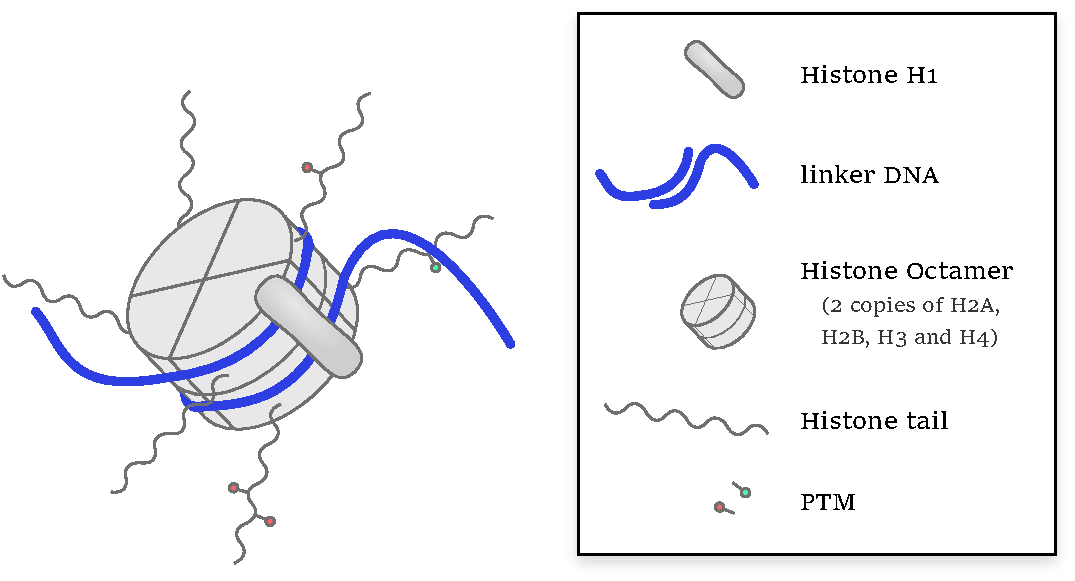
\includegraphics[width=0.7\textwidth]{annotated_nucleosome.pdf}
                \caption{schematic model of a nucleosome} % TODO complete caption.
                \label{img:nucleosome}
            \end{figure}
            %
            Chromatin can show higher order structure than the simple “beads on a string” variant. As such, nucleosomes that are not necessarily next neighbours along the DNA string can be in near proximity \cite{berg2015stryer, }.\\ % TODO The following higher order structures have been found by... % FIXME Source
            %
            Chromatin structure plays an important role in eukaryotic gene expression. Some DNA segments close to and on an actively transcribed gene are more easily accessible by proteins due to a locally more open chromatin structure. These chromatin regions are therefore called hypersensitive sites. \cite{cooper2017genome} Logically, the location of hypersensitive sites depends on the set of active genes and is thus cell-type and age specific \cite{berg2015stryer}.\\
            %
            The complex process of chromatin remodelling which leads to activation or repression of gene transcription comprises a vast multitude of agents and their interaction network is still not fully understood.\\
            %
        %
        %
        \subsection{Histone-modifying enzymes}
            %
            This thesis is based on one aspect of the chromatin remodelling machinery, namely histone-modifying enzyme complexes (HME). These complexes are able to covalently bind or remove chemical groups on amino acids (mostly R and K) at specific positions on the histone tail. The presence of these chemical groups changes the charge or polarity of the modified amino acids and thus influence the histone's affinity to the DNA. Histone-acetyltransferases (HATs), for instance, add an acetyl group to lysine, thus neutralizing the positive charge on the ammonium cation at neutral pH (see figure \ref{img:acetyllysineReaction}). This neutralization decreases the attraction to the negatively charged DNA backbone significantly resulting in the occurrence of a hypersensitive site. \cite{berg2015stryer} \\
            %
            \begin{figure}[htpb]
                \centering
                \vspace{.5cm}
                \schemestart
                    \arrow{0}[,0]
                    \chemname{\chemfig{!{lysine}}}{Lysine}\+\chemname{\chemfig{!{acetylcoa}}}{Acetyl-CoA} % TODO paint the acetyl-group red
                    \arrow[-90]
                    \chemfig{!{acetyllysine}}\+\chemfig{CoA-SH}\+\chemfig{H^+}
                \schemestop
                \vspace{.5cm}
                \caption{Acetylation of lysine. This reaction is catalysed by the HAT enzyme which by means of the cofactor acetyl coenzyme A (Acetyl-CoA) is able to trigger the transfer (substitution reaction in chemical terms) of an acetyl group onto the nitrogen atom in the side chain of lysine. The latter can be part of a histone tail.}
                \label{img:acetyllysineReaction}
            \end{figure}
            %
            Apart from the acetyl group, a multitude of other markers have been found on histone tails, e.g. methylation (one-, two and three-fold), phosphorylation, ubiquitylation, etc. These groups can entail gene transcription activation, silencing (repressing), or completely different purposes.\\ % FIXME source
            %
            This thesis will only feature acetylation as an activating modification and methylation as a silencing modification. Accordingly, the “state” of a nucleosome is defined as one of the following:
            %
            \begin{itemize}
                \item \textbf{unmodified}: There has been no PTM on any histone tail of the concerning nucleosome.
                \item \textbf{active}: Every PTM found on the concerning nucleosome enables gene activation. In this thesis, every one of these PTMs is an acetylation.
                \item \textbf{silent}: Every PTM found on the concerning nucleosome disables gene activation. In this thesis, every one of these PTMs is a methylation.
                \item \textbf{bivalent}: see \ref{sec:bivalency}
            \end{itemize}
            %
        %
        %
        \subsection{Bivalency}
            %
            \label{sec:bivalency}
            In pluripotent stem cells, nucleosomes have been found to contain both activating and silencing markers on histone tails of one and the same octamer. This bivalent state is believed to maintain a “poised state”, being ready to induce a gene expression cascade as soon as the silencing marker is removed. % FIXME source
            Others believe, that this bivalent state is connected to cell division and the ability of inheriting the active gene set for one daughter cell to induce differentiation while the other daughter cell remains a pluripotent stem cell \cite{schuettengruber2017genome}. % TODO is this right?
            %
            % TODO maybe add important enzyme types from biology here to later refer to them when explaining the models in ED
            %
        %
        %
    %
    %
    \section{Dynamic histone PTM models}
        %
        \subsection{(Solving the) chemical master equation}
            %
            The chemical master equation (CME) is the differential equation underlying the system that describes the time-dependent evolution of that system from a reactive point of view. Applied to the case at hand, we can establish the CME system made out of two equations for either the concentration of active (acetylated) and silent (methylated) nucleosome states.\\
            %
            In order to do this, one can establish the Langevin stochastic differential equation \cite{lemons1908paper} for each HME type, as was already done by Mayer in \cite{mayer2020langevin}. % TODO Langevin or CME?
            Eq. \ref{eqn:noncooperative} describe the noncooperative (see % TODO where do I explain cooperative?
            ) case for $a = \frac{A}{N}$ and $m = \frac{M}{N}$ with $A$ the number of acetylated nucleosomes, $M$ the number of acetylated nucleosomes and $N$ the total number of nucleosomes. $\alpha_i$ and $\beta_i$ are coefficients taking into account the types, association and dissociation ratios of the enzymes in the system.\\
            %
            \begin{subequations}
                \begin{align}
                    &\frac{\partial a}{\partial t} = \underbrace{- \alpha_1 a }_{\textrm{ac removal}} + \underbrace{ \alpha_2 a*(1-a-m) }_{\textrm{ac addition}}\\
                    &\frac{\partial m}{\partial t} = \underbrace{- \beta_1 m }_{\textrm{me removal}} + \underbrace{ \beta_2 m*(1-a-m) }_{\textrm{me addition}}
                \end{align}
                \label{eqn:noncooperative}
            \end{subequations}
            %
            Obviously, this would only be a usable model if the neighbour relations of the nucleosomes can be neglected. Given that the context from the enzyme rule sets is an important aspect of EpiDynast, an analytical solution of the CME would not be the best approximation. Also, depending on discrete numbers such as the number of nucleosomes in the string, the analytical solution of the CME as a continuous system, makes it even more unfitting as an approximation.\\
            %
            A more fitting system would be to establish and solve the CME for every nucleosome while the CME for nucleosome $i$ would depend on the number of neighbours equal to the biggest enzyme context in the system. So, if the rule set contains at least one rule including the next neighbours of the modified nucleosome $i$, the CME system would change to eqn. \ref{eqn:neighbourDependent}
            %
            \begin{subequations}
                \begin{align}
                    &\frac{\partial a_i}{\partial t} = - \alpha_1 (a_{i-1} + a_i + a_{i+1}) + \alpha_2 (a_{i-1} + a_i + a_{i+1})*(1-a-m)\\
                    &\frac{\partial m_i}{\partial t} = - \beta_1 (m_{i-1} + m_i + m_{i+1}) + \beta_2 (m_{i-1} + m_i + m_{i+1})*(1-a-m)
                \end{align}
                \label{eqn:neighbourDependent}
            \end{subequations}
            %
        %
        %
        \subsection{Gillespie's algorithm}
            %
            Gillespie's algorithm simulates the time evolution of a spatially homogenous molecular mixture under specification of the coupled reaction channels (i.e. association and enzymatic reaction with dissociation) based on stochastic chemical kinetics \cite{gillespie1976general, gillespie1992rigorous}. This is useful especially when solving the chemical master equation analytically is not ideal.\\
            %
            \begin{itemize}
                {
                    \color{red}
                    \item next-neighbours
                    \item rule-based, (paper from Arnold, Prohaska is basis for Nico's work, also basis for my work)
                    \item Gillespie's
                        \begin{itemize}
                            \item explain event based
                            \item steps from his paper
                        \end{itemize}
                    \item association and concentration are taken together.
                    \item enzyme types

                }
            \end{itemize}
            %
        %
        %
        \subsection{EpiDynast}
            %
            The software used in this thesis is \ed, developed by Herbig et al. % FIXME source for EpiDynast
            The main working mechanism may be outlined as follows: After defining enzyme rule sets and a starting nucleosome string (concerning their PTMs %TODO are these PTMs? DId I explain PTM?
            ), \ed simulates the stochastic time-dependent change of said modifications on the string, exactly one event at a time. The two events that can occur for each enzyme are either an association step or a reaction step that immediately entails dissociation of the enzyme from the nucleosome.\\
            %
            The enzyme rule sets simply describe a pattern (further on called “context” % TODO is the context including the site that is changed?
            ) on the string, that is then changed according to the rule. For instance, a linear acetylation extender enzyme % TODO either reference or put a picture
            would look for a pattern with two neighbouring nucleosomes, one acetylated and the other one unmodified and acetylate the latter.\\
            %
        %
        %

    %
    %
    \section{Epigenetic fitness landscapes} % TODO change title
        %
        \subsection{From landscape to vector field}
            %
            The term of epigenetic fitness landscape (referred to as landscape in the rest of this thesis) is mathematically defined as the triple $(V, \chi, f)$ where $V$ is a set of configurations, $\chi$ refers to the neighbouring relationship or similarity among the configurations and $f$ defines the fitness function of the landscape.\\ % FIXME source stadler
            %
            In this case, $V$ comprises the entirety of active, silent and unmodified state distributions along the nucleosome string, $\chi$ determines the modification of one nucleosome state, e.g. from silent to unmodified, or vice versa and $f$, which indicates the relative height or depth $f(v)$ of a specific configuration $v \in V$, is determined by all the association and dissociation rates, as well as the type of the enzymes in the system. In this specific landscape, the stochastic Gillespie's algorithm will always tend towards configurations (fix points) at the very base of landscape basins. These configurations are those, that are adopted in the majority of time steps throughout Gillespie's algorithm simulation.\\
            %
            \begin{figure}[htpb!]
                \centering
                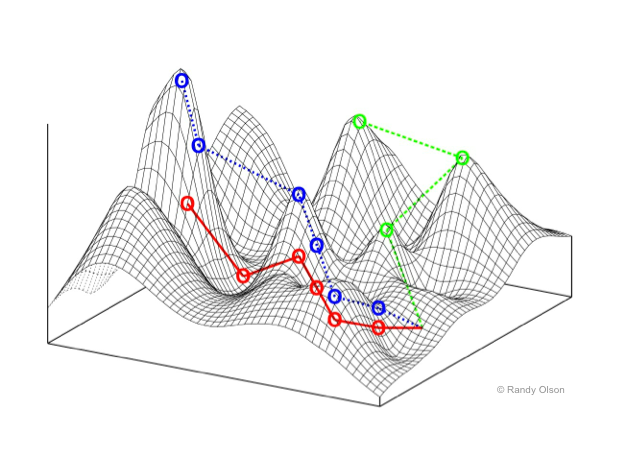
\includegraphics[width=0.7\textwidth]{prov_fitnessLandscape.png}
                \caption{Fitness landscape example and 2D projection.} % TODO change image to a self-made one. Maybe more intuitively usable for the case at hand
                % TODO insert tails and PTMs
                \label{img:fitnessLandscape}
            \end{figure}
            %
            Depending on the landscape, e.g. if there are deep and steep basins, it gets more and more difficult for the stochastic algorithm to exit the basin and adopt a configuration that lies outside. Each histone modifying enzyme thus induces a stability trend among the configurations which results in a vector field specific to each type of enzyme. In more complex systems with a multitude of different enzymes, these vector fields are combined % TODO no simple sum
            and create the resulting landscape at hand containing one or more fix points.\\
            %
            In this thesis,  there won't be any numerical values given to $f(v)$. However, by modifying the relative enzyme rate ratios, one can easily see that $f$ can change drastically resulting in it being much harder for the system to maintain a certain state or move along the shape of the landscape to switch from one state to another.\\ % TODO move this to discussion
            %
        %
        %
        \subsection{Enzyme types and bistability}
            %
            The number of fix points in the landscape can be analytically derived from the enzymes and their dependence on the frequency of nucleosome states (e.g. acetylation, methylation, ...) over time (see eqns. \ref{eqn:noncooperative}).\\
            %
            Mayer solved the equations analytically and found 4 critical values \cite{mayer2020langevin}: 3 fix points at $(0,0)$, $(0,1-\frac{\beta_1}{\beta_2})$, $(1-\frac{\alpha_1}{\alpha_2},0)$ and a separatrix that depends on the ratio between $\frac{\alpha_1}{\alpha_2}$ and $\frac{\beta_1}{\beta_2}$. The separatrix always has a gradient towards one of the non-trivial fix points. If $\frac{\alpha_1}{\alpha_2} = \frac{\beta_1}{\beta_2}$, the separatrix has no gradient.\\
            %
            \begin{figure}[ht!] % TODO include captions for vector graphs
                \centering
                \begin{minipage}{0.3\textwidth}
                    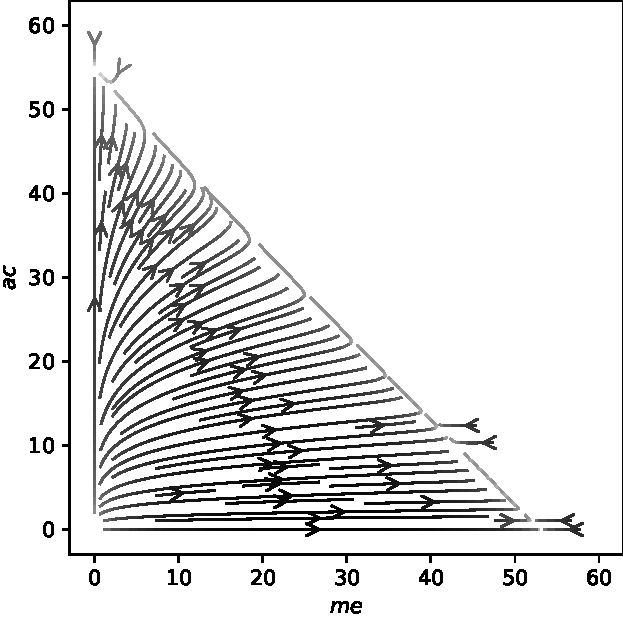
\includegraphics[width=\textwidth]{vectorfield_noncooperative_assymetric_monostable_ac.pdf}
                    \caption*{\small \textbf{(a)}}
                    \label{}
                \end{minipage}
                \begin{minipage}{0.3\textwidth}
                    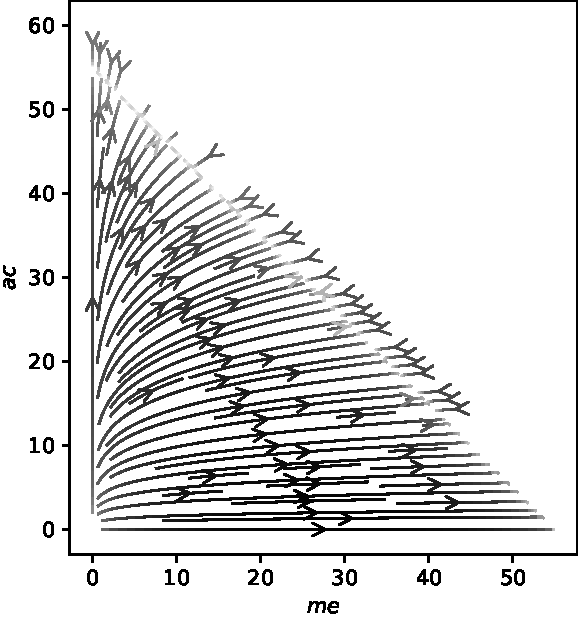
\includegraphics[width=\textwidth]{vectorfield_noncooperative_asymmetric_multistable.pdf}
                    \caption*{\small \textbf{(b)}}
                    \label{}
                \end{minipage}
                \begin{minipage}{0.3\textwidth}
                    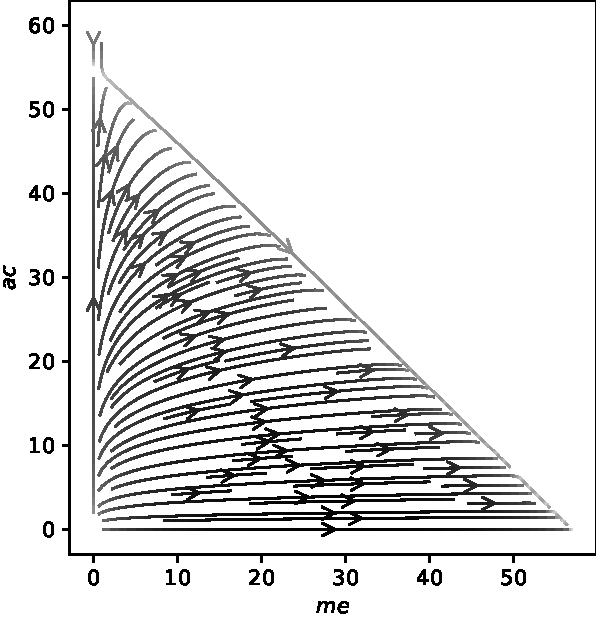
\includegraphics[width=\textwidth]{vectorfield_noncooperative_assymetric_monostable_me.pdf}
                    \caption*{\small \textbf{(c)}}
                    \label{}
                \end{minipage}
               \caption{\small  intervals.}
            \end{figure}
            %
            \begin{itemize}
                {
                    \color{red}
                    \item Can it be shown that the separatrix is only zero gradient if there is a null vector field?
                }
            \end{itemize} % TODO Can it be shown that the separatrix is only zero gradient if there is a null vector field?
            %
            In order for a dynamic histone PTM system to be bistable, the enzymes have to show cooperativity \cite{dodd2011barriers,sneppen2019theoretical,mayer2020langevin}. According to Sneppen \cite[][p.48]{sneppen2014models}, \enquote{cooperative binding means that the probability of occupying a state increases more than linearly with the concentrations of the binding molecules}.\\
            %
            In \cite{dodd2011barriers}, Dodd et al. specify the nature of cooperativity in order to reach ultrasensitivity\footnote{From Dodd et al. \cite{dodd2011barriers}: \enquote{Ultrasensitivity is a nonlinearity that magnifies any numerical advantage of one nucleosome type over another, allowing positive feedback to strongly push the system away from intermediate states and towards a large majority of one or other type.}} and thus a bistable system as follows\footnote{citations inside the quote changed their appearance in order to remain functional and to stylistically fit this work}:
            %
            \begin{quote}
                “Cooperativity can be direct, where two modified nucleosomes act together to recruit an enzyme to modify a third nucleosome \cite{3dodd2007theoretical,11sedighi2007epigenetic,15micheelsen2010theory}, or indirect, where each modified nucleosome catalyzes one of two separate modification reactions to fully convert a third nucleosome \cite{3dodd2007theoretical,13david2009inheritance}. A critical requirement for ultrasensitivity is that modified nucleosomes must act nonlocally, stimulating modification of nucleosomes located some distance away on the DNA. This long-range interaction is necessary for any nucleosome to be able to ‘sense’ the majority nucleosome type within the patch and cannot be provided by simple neighbor-to-neighbor contact \cite{3dodd2007theoretical,15micheelsen2010theory}.”
            \end{quote}
            %
            In other words, cooperativity can only be achieved by allowing the enzymes to detect more than one nucleosome that, in order to reach bistability, must not be a direct neighbour of the nucleosome to be (un)modified. This allows the modification that is superiorly prevalent over the whole string at that moment to be accounted for and recognized by the enzymes.\\
            %
            On a sidenote, the definition of cooperativity might seem slightly counterintuitive from a biochemical point of view, where the notion of cooperativity is strongly associated to be an asset of the enzyme \cite{cooperativityDefBritannica}. In contrast, according to Dodd et al., cooperativity is described as being a property of a set of nucleosomes being able to “cooperate” in order to recruit an enzyme and catalyse a reaction. Even though this not ideally put from a biochemical point of view, the mathematical implications still remain valid.\\ % TODO rephrase the notion of cooperativity from biochemical point of view
            %
            \begin{itemize}
                {
                    \color{red}
                    \item rephrase the biochemical side of cooperativity?
                }
            \end{itemize}
            %
            Mayer in \cite{mayer2020langevin} expressed the time dependent concentration of the modifications in the system in function of cooperative enzymes in the following differential equation system:
            %
            \begin{subequations}
                \begin{align}
                    &\frac{\partial a}{\partial t} = \underbrace{- \alpha_1 a }_{\textrm{ac rem}} + \underbrace{ \alpha_2 \frac{1}{n} a^2*(n-a-m) }_{\textrm{ac add}}\\
                    &\frac{\partial m}{\partial t} = \underbrace{- \beta_1 m }_{\textrm{me rem}} + \underbrace{ \beta_2 \frac{1}{n} m^2*(n-a-m) }_{\textrm{me add}}
                \end{align}
                \label{eqn:cooperative}
            \end{subequations}
            %
        %
        % TODO include Matilda's vector graphs
        \begin{itemize}
            {
                \color{red}
                \item Include Matilda's vector graphs
                    \begin{itemize}
                        \item Mark the fix points and separatrix
                    \end{itemize}
            }
        \end{itemize}
        %
    %
    %
    \section{Transition}
        %
        Although the mathematical foundation on whether a system can and cannot show bistability was already established, the execution in terms of building a model and rigorously identifying the influence of different factors within the model on the dynamics of a bistable system have, to my knowledge, not been explored yet.\\
        %
        Also, to date, bistable systems have not yet been modelled by means of a software that takes limited enzyme reach into account like \ed does.\\ % TODO remove space behind ED
        %
        This thesis will show exactly that. % TODO change sentence
        %
    %
    %
%
%

\chapter{Methods}
    \label{cha:methods}
    %
    \section{Chromatin Model}
    \label{sec:ChromatinModel}
        %
        The chromatin in \ed/ is modelled as an array of half-nucleosomes (for simplicity, the array of half-nucleosomes  is referred to as nucleosome string in the rest of the work), meaning that they only contain one tetramer of H2A, H2B, H3 and H4. The nucleosomes hold their respective position on the string so that the neighbour relations are fixed. That way, every nucleosome has exactly two neighbouring nucleosomes (in the cyclic case, see below) that stay the same throughout the entirety of a simulation. Furthermore, the nucleosomes are reduced to presence or absence of PTMs on their tails.
        %

        %
        The model in this work can even be reduced further, so that a nucleosome is modelled as 1 ($K27$) single amino acid which can be either acetylated (referred to as active) or monomethylated (referred to as silenced). Di- and trimethylation will not be featured in this work. Exceptionally, in \ref{sec:ResBivalency}, every nucleosome possesses 2 modifiable amino acids, called $K_x$ and $K_y$. All of these amino acids are monoacetylatable as well as monomethylatable. These two modifications are mutually-exclusive one one amino acid. However, $K_x$ and $K_y$ can very well contain opposing modifications in which case the concerning nucleosome will be referred to as bivalent.\\
        %

        %
        The nucleosome string is either modelled to be non-cyclic (as done in \ref{sec:ResNon-cooperative} and \ref{sec:ResNonCyc}) or cyclic (\ref{sec:ResBistableSwitching} to \ref{sec:ResBivalency}). In the cyclic case, the enzymes' context can include nucleosomes from the start as well as the end of the string simultaneously. In the non-cyclic case, the first and last nucleosome logically only have one neighbour.
        %

        %
        The non-cyclic models contain 60 nucleosomes whereas the cyclic ones only contain 40 nucleosomes in order to reduce computation time and storage space.
        %

        %
        The starting state for every simulation in this work is a completely unmodified nucleosome string. As long as there are random adders in the system (which is the case for every system featured in this work), the completely unmodified string logically is an unstable configuration which does not offer any sort of bias in the direction of acetylation or methylation respectively, hence the choice of an entirely unmodified starting state. The time it takes the system to adjust to establishing a modified string is negligible compared to the total time of one simulation run.
        %
    %
    %
    \section{Enzyme models}
        %
        \subsection{Enzymes in \ed/}
            %
            The enzymes in \ed/ are mainly described by their reaction nature, the context needed in order to perform the reaction, their association and their dissociation rate. The reaction nature defines the change that the enzyme is performing on the nucleosomes' modifications. Generally, the enzymes are either modification adders or modification removers (see \ref{subsec:EnzymeTypes} for details).
            %

            %
            The enzyme's context can be defined as the set of one or more nucleosome PTMs that must be present in a precisely determined neighbour-relation to the nucleosome that is intended to be changed. If the enzyme finds the needed context to be unfitting, the reaction of this enzyme with the determined nucleosome is not taken into the propensity sum of that simulation step (see the explanation of Gillespie's algorithm in \ref{subsec:Gillespie}). Random enzymes have a context which exclusively contains the one nucleosome that is about to be modified by the enzyme (see \ref{subsec:EnzymeTypes} for details). The reaction nature and context are defined together by a specific set of (possibly multiple) rules for each enzyme.
            %

            %
            The association rate together with the enzyme's concentration define the enzyme's affinity to its substrate. The dissociation rate in turn defines the enzyme's speed concerning reaction and diffusion away from the modified nucleosome. On a sidenote, Gillespie's algorithm and thus \ed/ offer the possibility to model concentration depletion effects. This was not used in this work. Accordingly, all enzymes were assumed to be equally and infinitely available in the simulation.
            %

            %
            The enzyme rule sets as well as their rates are defined symmetrically throughout the entirety of the simulations that were done for this work. Thus, for instance, every rule defining the addition of an acetyl group to a nucleosome next to one that already has an acetyl group is defined in either direction on the string and has a methylation counterpart at equal rates.
            %
        %
        %
        \subsection{Enzyme types}
            \label{subsec:EnzymeTypes}
            %
            A short summary of all enzyme types featured in this work can be found in tab. \ref{img:enzymeTypeSummary}.
            %

            %
            \subsubsection*{Linear enzymes}
                %

                \begin{figure}[htpb!]
                    \centering
                    \begin{minipage}[t][5cm]{\textwidth}
                        \begin{minipage}{0.15\textwidth}
                            \caption*{\small \textbf{(a)}}
                        \end{minipage}
                        \begin{minipage}{0.8\textwidth}
                            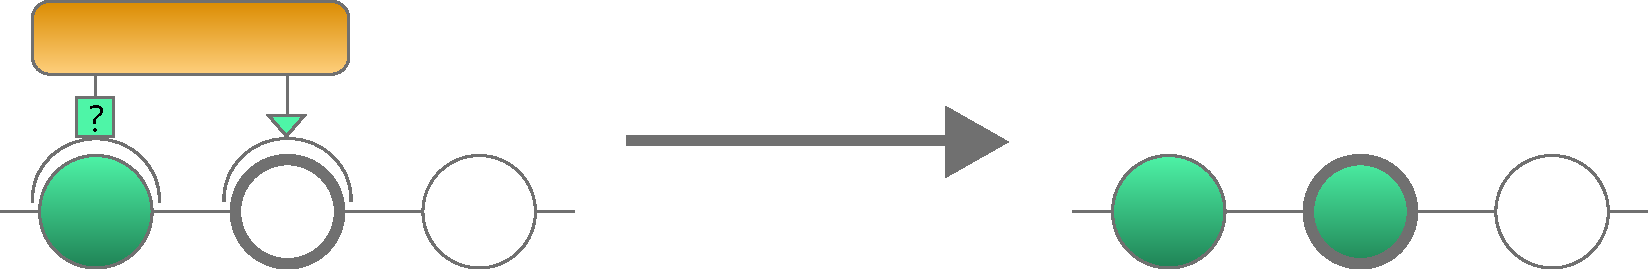
\includegraphics[width=\textwidth]{enzymes/linear_a.pdf}
                        \end{minipage}
                        \vfill
                        \begin{minipage}{0.15\textwidth}
                            \caption*{\small \textbf{(b)}}
                        \end{minipage}
                        \begin{minipage}{0.8\textwidth}
                            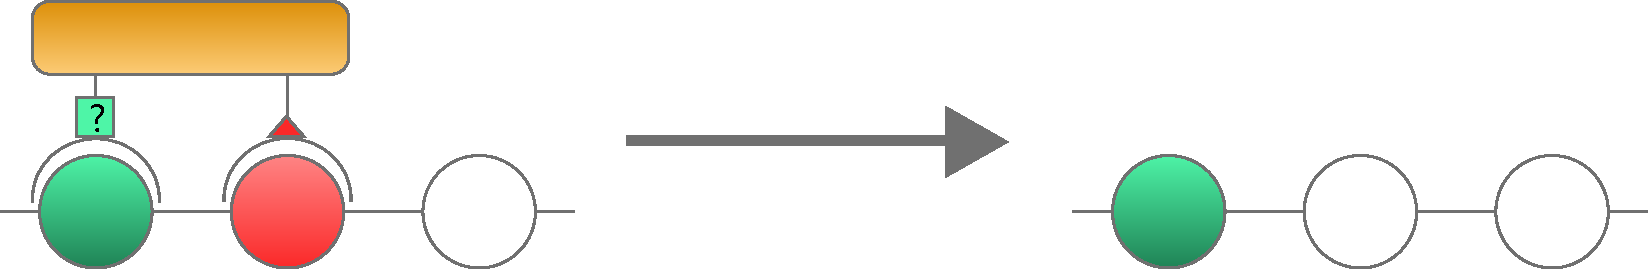
\includegraphics[width=\textwidth]{enzymes/linear_b.pdf}
                        \end{minipage}
                    \end{minipage}
                    \caption{Simplified model of linear enzyme acetylation addition \textbf{(a)} and methylation removal \textbf{(b)} reactions. Acetylated nucleosomes are coloured in green, methylated nucleosomes are red and colourless ones are unmodified. The reactions shown are also defined in the rule set to occur in the opposite direction. Linear enzymes in favour of methylation extension (or acetylation deletion) work analogically.}
                    \label{img:linearEnzymes}
                \end{figure}
                %

                %
                Linear enzymes are used to extending sites containing a specific modification (e.g. acetylation, see fig. \ref{img:linearEnzymes}) by either propagating said modification from nucleosome to neighbouring unmodified nucleosome or by deleting an opposing modification next to a nucleosome with the desired modification. They exclusively have next neighbour reach.
                %
            %
            %
            \subsubsection*{Cooperative enzymes}
                \label{subsubsec:coopEnzymes}
                %
                \begin{figure}[htpb!]
                    \centering
                    \begin{minipage}[t][3cm]{\textwidth}
                        \begin{minipage}{0.15\textwidth}
                            \caption*{\small \textbf{(a)}}
                        \end{minipage}
                        \begin{minipage}{0.8\textwidth}
                            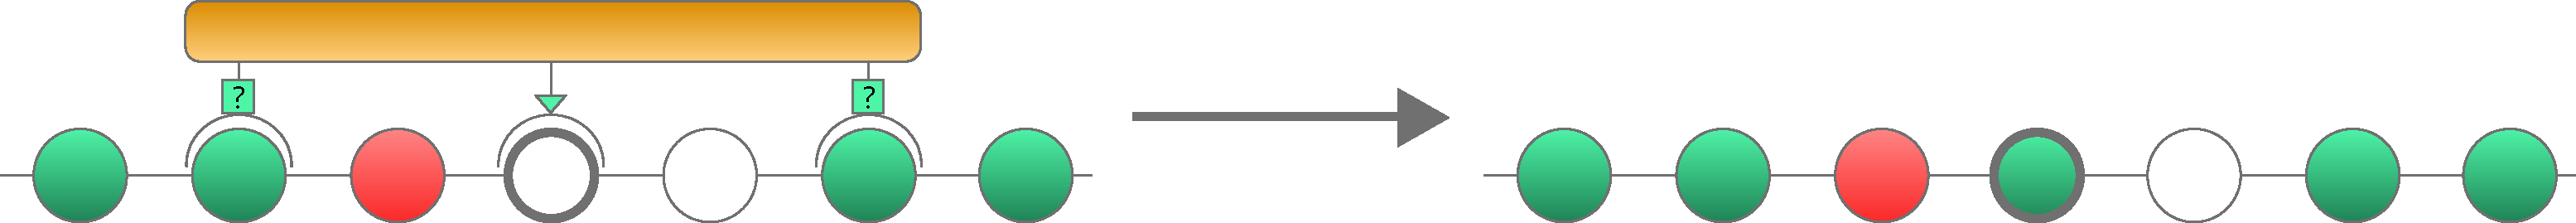
\includegraphics[width=\textwidth]{enzymes/coop_a.pdf}
                        \end{minipage}
                    \vfill
                        \begin{minipage}{0.15\textwidth}
                            \caption*{\small \textbf{(b)}}
                        \end{minipage}
                        \begin{minipage}{0.8\textwidth}
                            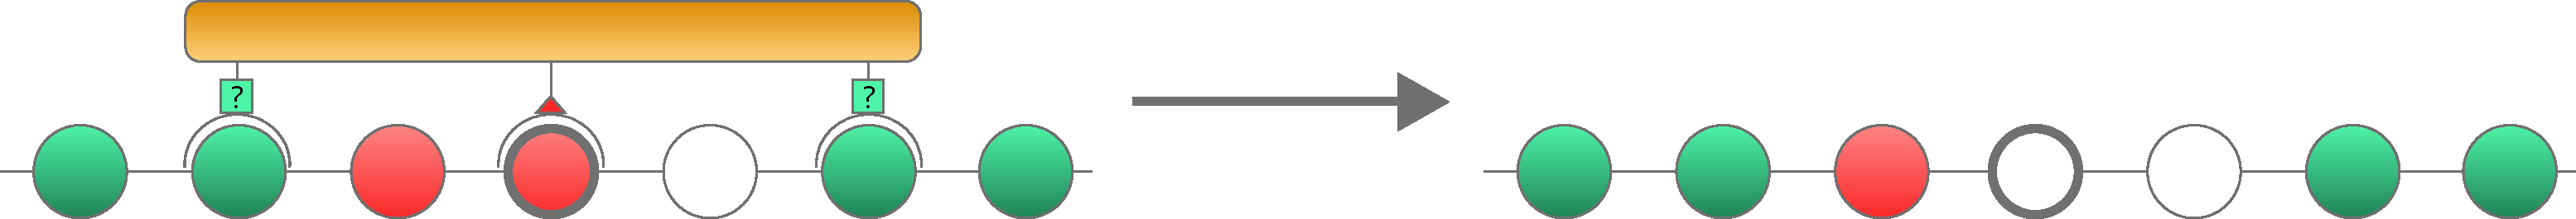
\includegraphics[width=\textwidth]{enzymes/coop_b.pdf}
                        \end{minipage}
                    \end{minipage}
                    \caption{Simplified model of cooperative enzyme acetylation addition \textbf{(a)} and methylation removal \textbf{(b)} reactions. Acetylated nucleosomes are coloured in green, methylated nucleosomes are red and colourless ones are unmodified. The reactions shown are also defined in the rule set to occur in the opposite direction. Cooperative enzyme methylation  addition and acetylation removal work analogically.}
                    \label{img:coopEnzymes}
                \end{figure}
                %

                %
                Cooperative enzymes generally read the state of two different nucleosomes on the string and write to or remove a modification from a third nucleosome. It is important to note that the two nucleosomes that are read do not need to have any next-neighbour relation to the one the enzyme is modifying.  Thus, to some extent, these enzymes, unlike any other enzyme featured in this work, take the global modification trend on the string into account: if many nucleosomes are acetylated, then cooperative enzymes in favour of acetylation (meaning cooperative acetylation adders and cooperative methylation removers) are more active which, in turn, reinforces the acetylation distribution on the string.
                %

                %
                The cooperative enzymes in this work are implemented in a way that they are always reading two nucleosomes that are equally far away from the nucleosome the enzyme wants to modify (see fig. \ref{img:coopEnzymes}).
                %

                %
                The notion of 'space' of a cooperative enzyme defines the context reach of said enzyme. For instance, a cooperative adder with a reach of 3 will read the nucleosome it wants to write on and ignore the 3 next neighbours of this nucleosome. It will only read the 4th nucleosomes situated to the left and the right of the first one. Accordingly, a cooperative enzyme which reads the next neighbours of the nucleosome to write on by definition has a reach of 0.
                %


            %
            %
            \subsubsection*{Random enzymes}
                %
                Random adder and remover enzymes serve as noise in the system. As these enzymes act on one single nucleosome, they do not take into account any other nucleosomes on the string. As such, random adders are the only enzymes featured in this work that are able to modify a nucleosome on an otherwise completely unmodified string.
                %
                \begin{figure}[htpb!]
                    \centering
                    \begin{minipage}[t][5cm]{\textwidth}
                        \begin{minipage}{0.15\textwidth}
                            \caption*{\small \textbf{(a)}}
                        \end{minipage}
                        \begin{minipage}{0.8\textwidth}
                            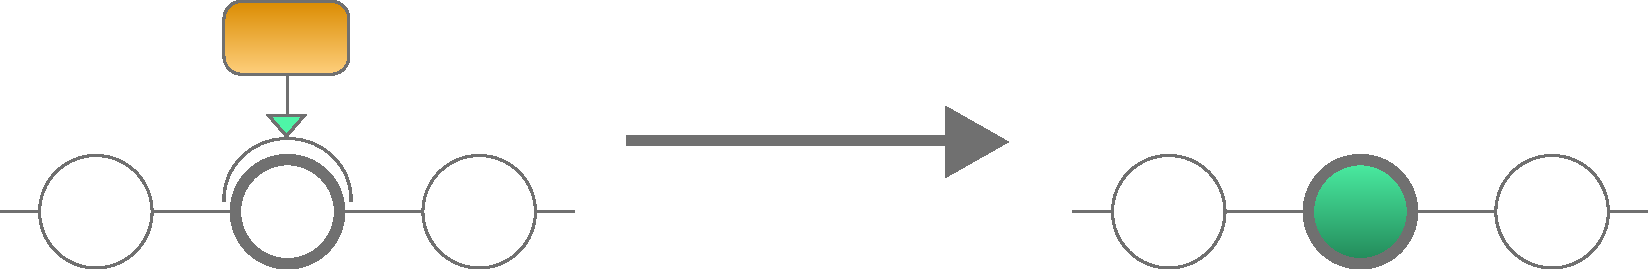
\includegraphics[width=\textwidth]{enzymes/random_a.pdf}
                        \end{minipage}
                        \vfill
                        \begin{minipage}{0.15\textwidth}
                            \caption*{\small \textbf{(b)}}
                        \end{minipage}
                        \begin{minipage}{0.8\textwidth}
                            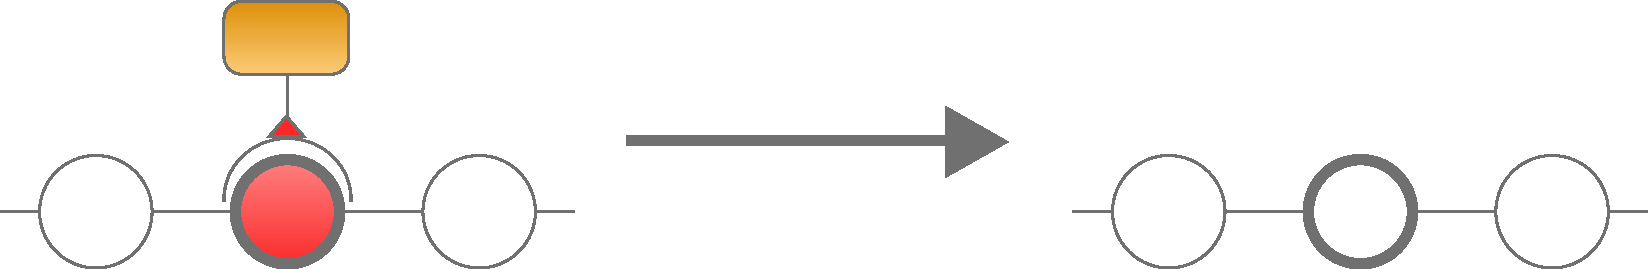
\includegraphics[width=\textwidth]{enzymes/random_b.pdf}
                        \end{minipage}
                    \end{minipage}
                    \caption{Simplified model of random enzyme acetylation addition \textbf{(a)} and methylation removal \textbf{(b)} reactions. Acetylated nucleosomes are coloured in green, methylated nucleosomes are red and colourless ones are unmodified. Random enzyme methylation addition and acetylation removal work analogically.}
                    \label{img:randomEnzymes}
                \end{figure}
                %

                %
                Random enzymes still have a context, as for example a random methylation adder cannot bind to any already modified nucleosome, only to an unmodified one. Given that any nucleosome can be targeted by a specific random enzyme at any moment, these enzymes' association rate should be smaller than the other ones' in the system by many orders of magnitude.
                %

                %
                Random enzymes are not only “enzymes” in the true sense of the word when compared to the biological side of the model. They also exist in order to mimic the “noise” that is associated with such systems.
                %

                %
                \begin{itemize}
                    {
                        \color{red}
                        \item Explain PRC2 with JARID2 DNA-binding TF subcomponent?
                    }
                \end{itemize}
                %
                %
            %
            %
            \subsubsection*{Completer enzymes}
                %
                \begin{figure}[htpb!]
                    \centering
                    \begin{minipage}[t][10cm]{\textwidth}
                        \begin{minipage}{0.15\textwidth}
                            \caption*{\small \textbf{(a)}}
                        \end{minipage}
                        \begin{minipage}{0.8\textwidth}
                            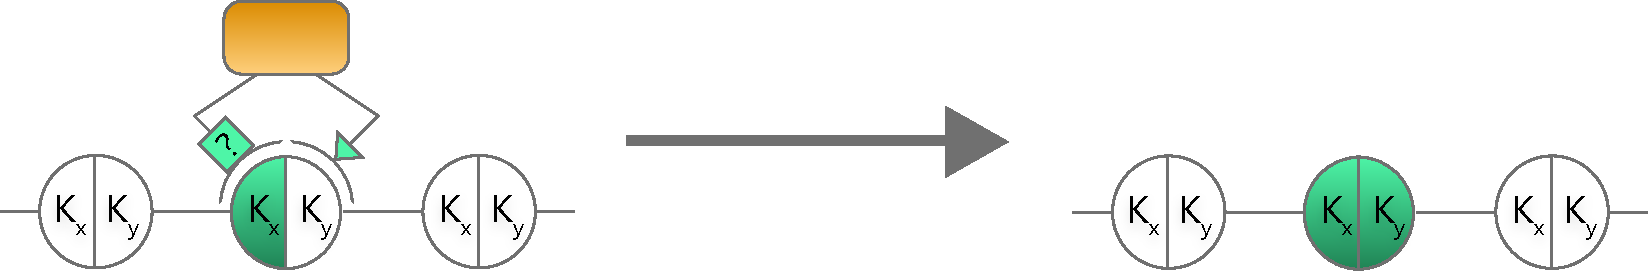
\includegraphics[width=\textwidth]{enzymes/completer_total_a.pdf}
                        \end{minipage}
                        \vfill
                        \begin{minipage}{0.15\textwidth}
                            \caption*{\small \textbf{(b)}}
                        \end{minipage}
                        \begin{minipage}{0.8\textwidth}
                            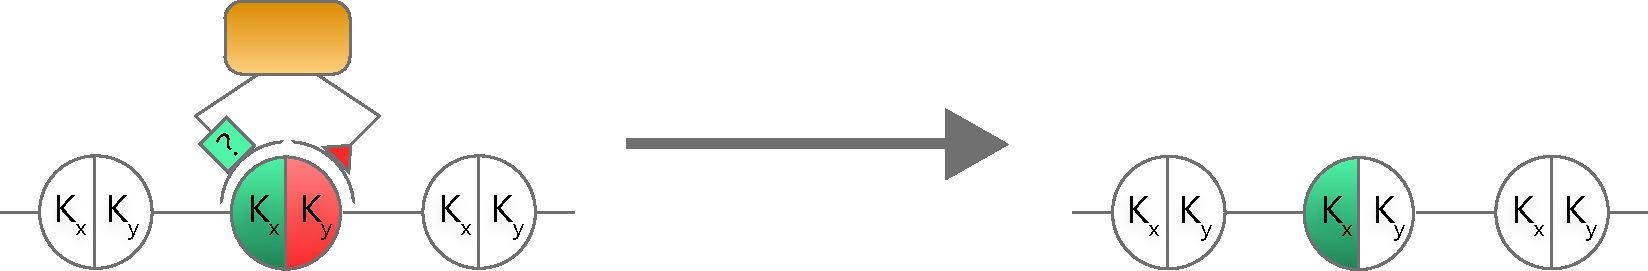
\includegraphics[width=\textwidth]{enzymes/completer_total_b.pdf}
                        \end{minipage}
                        \vfill
                        \begin{minipage}{0.15\textwidth}
                            \caption*{\small \textbf{(c)}}
                        \end{minipage}
                        \begin{minipage}{0.8\textwidth}
                            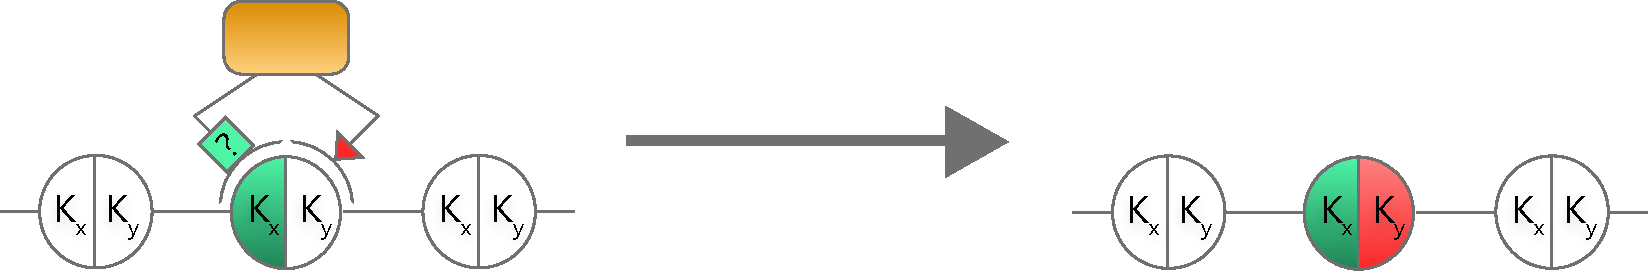
\includegraphics[width=\textwidth]{enzymes/completer_biv_a.pdf}
                        \end{minipage}
                        \vfill
                        \begin{minipage}{0.15\textwidth}
                            \caption*{\small \textbf{(d)}}
                        \end{minipage}
                        \begin{minipage}{0.8\textwidth}
                            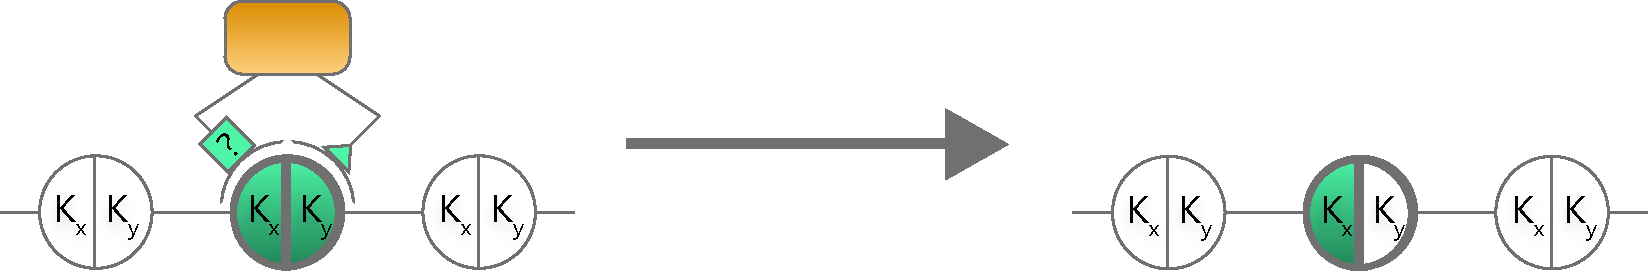
\includegraphics[width=\textwidth]{enzymes/completer_biv_b.pdf}
                        \end{minipage}
                    \end{minipage}
                    \caption{Simplified model of the enzyme acetylation addition and removal reactions. \textbf{(a)} and \textbf{(b)} show reactions in favour of “total” states, which means that they enforce one single type of modification on a nucleosome, while \textbf{(c)} and \textbf{(d)} respectively show addition and removal reactions favouring bivalent nucleosomes. The reactions shown are also defined in the rule set to occur in the opposite direction. Total enzyme methylation addition and acetylation removal work analogically.}
                    \label{img:completerEnzymes}
                \end{figure}
                %

                %
                Completer enzymes are the only enzymes featured in this work which modify two different amino acids on one single nucleosome. These amino acids are exemplarily called $K_x$ and $K_y$ and, like the amino acid on the other nucleosomes, are both methylatable and acetylatable. Completer enzymes only act on one single nucleosome. They read one amino acid and write to or remove from the other one. As such, these enzymes are used in order to reinforce the generation of bivalent states or “total” (fully acetylated or fully methylated) states among the nucleosomes.
                %

                %
                Completer enzymes have no known scientific background. They only serve the purpose of analysing the system dynamics when provoking bivalency or total states in the system.
                %
            %
            %
        %
        %
        \subsection{Enzyme rule sets}
            %
            This subsection provides an overview of the different enzyme rule sets used in the different simulations featured in this work. The rule sets are almost always kept constant throughout every section in the 'Results' chapter respectively. The enzyme rule sets used are the following (depending on the reader's preference, the rule sets can also be looked up in tab. \ref{tab:EnzymeRuleSets}):
            %

            %
            % \begin{itemize}
            %     {
            %         \item 3.1: linear adders, linear removers, random adders, random removers
            %         \item 3.2: cooperative adders, cooperative removers (not for some), random adders, random removers (non-cyclic)
            %         \item 3.3: cooperative adders, cooperative removers (not for some), random adders, random removers (cyclic)
            %         \item 3.4: cooperative adders, random adders, random removers (cyclic)
            %         \item 3.5: cooperative adders, random adders, random removers (cyclic)
            %         \item 3.6: (cyclic)
            %             \begin{itemize}
            %                 \item BivalentBistability: cooperative adders (0-5 for all), cooperative removers, random adders, random removers,
            %                 \item FavTotal: total completers, total self removers, random adders, random removers
            %                 \item FavBivalency: bivalent completers, bivalent self removers, random adders, random removers
            %             \end{itemize}
            %     }
            % \end{itemize}
            %

            %
            \begin{table}
                \centering
                \caption{Summary on whether an enzyme type was included in the designated experiment presented in the indicated 'Results' section. The \textbf{X} indicates that the enzyme type was featured, while the \textbf{~} indicates that there were some runs in this section that featured the referring enzyme type, while other runs in this same section did not. The explanation as to why this was done can be found in the respective sections.}
                \begin{tabular}{l|c|c|c|c|c|c|c|c|}
                                            & \multirow{2}{*}{3.1} & \multirow{2}{*}{3.2} & \multirow{2}{*}{3.3} & \multirow{2}{*}{3.4} & \multirow{2}{*}{3.5} & \multicolumn{3}{c|}{3.6}                        \\
                                            &                      &                      &                      &                      &                      & BivBist & Total      & Bivalent    \\\hline
                random adders               & \textbf{X}           & \textbf{X}           & \textbf{X}           & \textbf{X}           & \textbf{X}           & \textbf{X}          & \textbf{X} & \textbf{X}  \\\hline
                random removers             & \textbf{X}           & \textbf{X}           & \textbf{X}           & \textbf{X}           & \textbf{X}           & \textbf{X}          & \textbf{X} & \textbf{X}  \\\hline
                linear adders               & \textbf{X}           &                      &                      &                      &                      &                     &            &             \\\hline
                linear removers             & \textbf{X}           &                      &                      &                      &                      &                     &            &             \\\hline
                cooperative adders          &                      & \textbf{X}           & \textbf{X}           & \textbf{X}           & \textbf{X}           & \textbf{X}          &            &             \\\hline
                cooperative removers        &                      & \textbf{~}          & \textbf{~}          &                      &                      & \textbf{~}         &            &             \\\hline
                bivalent completer adders   &                      &                      &                      &                      &                      &                     &            & \textbf{X}  \\\hline
                bivalent completer removers &                      &                      &                      &                      &                      &                     &            & \textbf{X}  \\\hline
                total completer adders      &                      &                      &                      &                      &                      &                     & \textbf{X} &             \\\hline
                total completer removers    &                      &                      &                      &                      &                      &                     & \textbf{X} &             \\\hline
                cyclic                      &                      &                      & \textbf{X}           & \textbf{X}           & \textbf{X}           & \textbf{X}          & \textbf{X} & \textbf{X}  \\\hline
                non-cyclic                  & \textbf{X}           & \textbf{X}           &                      &                      &                      &                     &            & \\\hline
                \end{tabular}
                \label{tab:EnzymeRuleSets}
            \end{table}
            %
        %
        %
    %
    %
    \section{Simulation details}
    \label{sec:simulationDetails}
        %
        The input files for every result section's \ed/ simulations can be found at \source. In general, every \ed/ run needs 3 files: a \textit{statefile}, a \textit{rulefile} and a \textit{paramfile}. The \textit{statefile} contains the starting state of the nucleosome string. The \textit{rulefile} contains all specifications to the enzymes: their contexts, the modification pattern, the association rate and the dissociation rate. The \textit{paramfile} holds general information about the simulation itself with the most important one being the simulation time. This numeric parameter sets the exit condition for the algorithm.
        %

        %
        The simulation time changes significantly between some runs. This is due to Gillespie's algorithm's event-based time approach. Changing the enzyme set can result in a significantly different number of possible reactions during the simulation which can lead to very short simulation step numbers. Thus, in order to grant statistically significant runs, the simulation time was increased for certain runs, where the overall run time was empirically found to be too short.
        %

        %
        Furthermore, for reasons of performance and storage space, the graphs included in the results section were made from simulations with different simulation time. Preprocessing for the heatmaps was significantly more expensive than the other plots. Therefore, heatmaps were generated from \textit{short} runs, whereas the other plots were generated from \textit{long} runs. Meaning:
        %

        %
        \begin{itemize}
            \item \textit{short}: Every step (event) is plotted and metadata are used to plot association numbers and relative binding time (resulting in heatmaps).
            \item \textit{long}: Only every 1000th step is plotted. Given that the system is chaotic thanks to the random nature of the algorithm, regular plotting (f. ex. every 1000th data point) results in a smoothing of the histogram because the chosen data points are more representative for the underlying distribution.
        \end{itemize}
        %

        %
        The different simulation parameters for the runs featured in this work are summarized in \ref{tab:simulationParametersSummary}.
        %
    %
    %
%
%
\chapter{Results}
    \label{cha:results}
    %
    \section{Non-cooperative enzymes do not entail bistable systems}
        %
        Considering a system without cooperative enzymes, that thus only contains enzymes with a context that includes the next neighbours at most, bistability can not be achieved. Indeed, fig. \ref{img:linearCase} discloses a monostable system, as the histogram shows an unimodal distribution throughout the simulation.\\ % Link to more simulation results in appendix?
        %
        \begin{figure}[htpb!]
            \centering
            % \includegraphics[width=0.7\textwidth]{}
            \caption{Boring monostable case. The rule sets used the following enzymes: ? (Rates and additional runs can be found in Appendix.)}
            \label{img:linearCase}
        \end{figure}
        %
        Fig. \ref{img:linearCase} exemplarily shows that the total number of active and silent states ambulate around one same value. In fig. % TODO make figure
        , one can see that even though the overall number of active and silent states changes over time, the overall order in the system stays invariant as the only enzymatic actions are taking place in between the two modification areas at their border. % TODO Discussion: In a case of symmetrical rule set rates, the border will always stay in the middle, because stochastics?
        %
        \begin{itemize}
            {
                \color{red}
                \item Include a boring graph that does not change much. Emphasis on the histogram.  % _,.-^-.,_
                \item Renew the graphs
                    \begin{itemize}
                        \item Gillespie time instead of step number on x-axis
                        \item remove bivalency window where it isn't needed
                        \item print (not plot) the total step number and indicate it in the caption
                        \item remove title
                    \end{itemize}
                \item run the heat map plots on these in order to see if there are to areas or if they are homogeneously mixed
            }
        \end{itemize}
        %
        %
    \section{cooperative enzyme case}
        %
        \begin{itemize}
            {
                \color{red}
                        \item non-cyclic
                            \begin{itemize}
                                \item high vs. low dissociation rate
                                \item Explain bistability and low frequency switching
                            \end{itemize}
                        \item cyclic
                            \begin{itemize}
                                \item case without switchings
                                \item case with frequent switchings
                                    \begin{itemize}
                                        \item normal bistable
                                        \item compare to lower reach
                                    \end{itemize}
                            \end{itemize}
            }
        \end{itemize}
        %
    %
    %
    \section{Bivalency} % TODO Should I include these  cases into the others above? Pro: I don't find anything ground-breaking here. Con: I have an entirely different system which might lead to confusion
        %
        \begin{itemize}
            {
                \color{red}
                \item Here, we are at Kx+Ky
                \item Two systems that either favour bivalency or total active/silent states
                \item Frequent switching and bivalency
            }
        \end{itemize}
        %
    %
    %
    % \section{Impact of dissociation rate on amount of noise}
    %     %

    %     %
    % %
    % %
    % \section{Bistability in EpiDynast}
    %     %
    %     \begin{itemize}
    %         {
    %             \color{red}
    %             \item play with spacing and rates, dynamic spacing functionality added to program (pseudo-code in appendix or...)
    %             \item Make enzyme reach smaller. What happens to the rapidly switching system?
    %         }
    %     \end{itemize}
    %     %
    % %
    % %
    % \section{(Bistability vs. Bivalency)}
    %     %

    %     %
    % %
    % %
    % \section{Border effects in \ed}
    %     %
    %     \begin{itemize}
    %         {
    %             \color{red}
    %             \item The process of bistable switchings
    %             \item influential factors on bistable switching
    %         }
    %     \end{itemize}
    %     %
    % %
    % %
    % \section{(A memory capable system)}
    %     %
    %     \begin{itemize}
    %         {
    %             \color{red}
    %             \item either as goal ("this is why I want to get more frequent switchings")
    %             \item or as a means to analyze and apply statistics to switchings (many many runs)
    %             \item I could also run with bigger time intervals)
    %         }
    %     \end{itemize}
    %     %
    % %
    % %
%
%
\chapter{Discussion}
    \label{cha:discussion}
    %
    \begin{itemize}
        {
            \color{red}
            \item Summarize the findings.
        }
    \end{itemize}
    %

    %
    \section{Conditions for bistability}
        %
        Hence, even though, there is evidence about the occurrence of fully activated and fully silenced states, this is only a statistical effect. The probability of the system being in an intermediate state is way higher, which disqualifies this system of being an effective "switch" between two extreme states.
        %

        %
        \begin{itemize}
            {
                \color{red}
                \item Bistability (condition: cooperativity) (Explain difference between biological and Sneppen coop.) (Errors in Sneppen's insights on the topic)
                \item Impact of dissociation rate: The dissociation rate was not taken into account for most of the simulations. Setting one and the same high dissociation rate that hardly competes with the association rates of the enzymes smoothens the nucleosome state histograms and thus reduces noise in the system. In terms of epigenetic landscapes, a variable dissociation rate would introduce much complexity into the system, as the number of relevant states would increase. This is the case because every state now would not only be sufficingly described by its modification states but also by the number and type of enzymes bound to the nucleosomes. However, even though the complexity increases significantly, there would not be any inherent biological experience gain from this.
            }
        \end{itemize}
        %
    %
    %
    \section{Proposed mechanism for bistable switching}
        %
        \subsection{Bistable switching: a biologically useful phenomenon}
            %

            %
        %
        %
        \subsection{cyclic}
            %

            %
        %
        %
        \subsection{non-cyclic}
            %
            \begin{itemize}
                {
                    \color{red}
                    \item A state seed will immediately be extinguished by an opposing cooperative remover. In order to prevent this, there are two possibilities:
                        \begin{itemize}
                            \item Build the seed in a corner where the coop Remover cannot be active
                            \item Remove coop Removers
                        \end{itemize}
                }
            \end{itemize}
            %
        %
        %
    %
    %
%
%

\chapter{Outlook}
\label{cha:outlook}




\section{Make \ed/ account for recent biological findings}
    %
    Schuettengruber et al. in \cite{schuettengruber2017genome} (p44f) % TODO remove page number
    explain that PREs (Polycomb response elements) are responsible for the chromatin forming loops (TADs = topologically associating domains) and are thus able to form large silenced areas of condensed chromatin. These 3D-formations are critical for HOX gene regulation. It is also known that many active gene promoters interact with their enhancers and other promoters in a 3d-fashion. \cite{javierre2016lineage} These findings suggest that it might be beneficial for \ed/ simulations to further explore possibilities to emulate fixed and dynamic 3D interactions within the nucleosome string.
    %
%
%
\section{Explore recently discovered non-cooperative edge case}
    %
    \begin{figure}[htpb!]
        \centering
        \includerunplot{Results/outlook/StrongExtenders_cyclic_1_runHistoryPlot.pdf}
        \caption{Absolute number of nucleosome states (active in green, silent in red) during the course of one long simulation (about 3.9 million reaction steps). The enzyme rule set contains linear extenders, linear removers, random adders and random removers. The rule set does not contain cooperative enzymes.}
        \label{img:outlook_nonCoop}
    \end{figure}
    %

    %
    A quite unexpected result was found in a system of exclusively non-cooperative enzymes at a very specific association rate ratio summarized in table \ref{img:enzymeRatesPeculiarCase}. The state adoption in this system resembles bistable behaviour as can be seen in fig. \ref{img:outlook_nonCoop}. One can clearly see that there are two very distinct peaks at complete activation and complete silencing of the nucleosome string. Even though this system seems to be bistable, it shows one very important difference to the bistable systems explored earlier in this work: the lack of variance around the peaks in the histogram.
    %

    %
    \begin{table}[htbp!]
        \caption{Enzyme types that are included in the rule set for the run illustrated in fig. \ref{img:outlook_nonCoop} with their respective association rates. All enzymes' dissociation rates are at an equal rate of 100000. The enzyme rule set is symmetrical, which means that every enzyme type exists in favour of acetylation as well as methylation at equal rates respectively.}
        \begin{center}
            \begin{tabular}{l r}
                \hline
                \textbf{enzyme type} & \textbf{association rate} \\
                \hline
                random adder & 100 \\
                random remover & 2 \\
                linear extender & 20000 \\
                linear remover & 20000 \\
                \hline
            \end{tabular}
        \end{center}
        \label{img:enzymeRatesPeculiarCase}
    \end{table}
    %

    %
    As stated earlier, the histograms' peak variance can be understood as the area where the system has a more or less strong tendency to return to the peak's state. Or, in mathematical terms, the variance is the area in the system's underlying vector field that points in the critical point's direction.
    %

    %
    This behaviour is not observed in the non-cooperative case described in fig. \ref{img:outlook_nonCoop}. Thus, one single opposite modification added randomly to the string entails the system's return to a random walk. As the term “stability” describes a state's resistance against small deviations and the addition of one single modification is nothing more than an atomic step for this system % TODO: maybe refer to step function of fitness landscape
    one can say, that this non-cooperative case does not qualify as being bistable in the true sense of the word.
    %

    %
    Nonetheless, it is an interesting phenomenon worth exploring, as it remains debatable if “true bistability” is really needed in the biological context.
    %

%%%----------------------------------------------------------
\appendix                                         % appendix
%%%----------------------------------------------------------

\chapter{Specifications}
    \label{app:RunSpec}
    %

    %
    \section{Exemplary \ed/ run files}
        %
        \subsection{State file}
            \label{app:statefile}
            %
            \lstinputlisting[language=XMLnew]{xml/statefile.xml}
            %
        %
        %
        \subsection{Rule file}
            \label{app:rulefile}
            %
            \lstinputlisting[language=XMLnew]{xml/rulefile.xml}
            %
        %
        %
        \subsection{Param file}
            \label{app:paramfile}
            %
            \lstinputlisting[language=XMLnew]{xml/paramfile.xml}
            %
        %
        %
    %

    %
    \newpage
    \section{Summary of enzyme types}
        %

        %
        \begin{table}[htbp!]
            \caption{Summary of all the enzyme types that are referenced in this work. It is important to mention, that, for reasons of comprehensiveness, this table exemplarily only includes the rules which are in favour of acetylation (i.e. acetylation adders and methylation removers). However, every enzyme set used in this work is completely symmetrical. This means that if an enzyme set contains a linear acetylation adder it also contains a linear methylation adder at equal association and dissociation rates respectively and so forth.}
            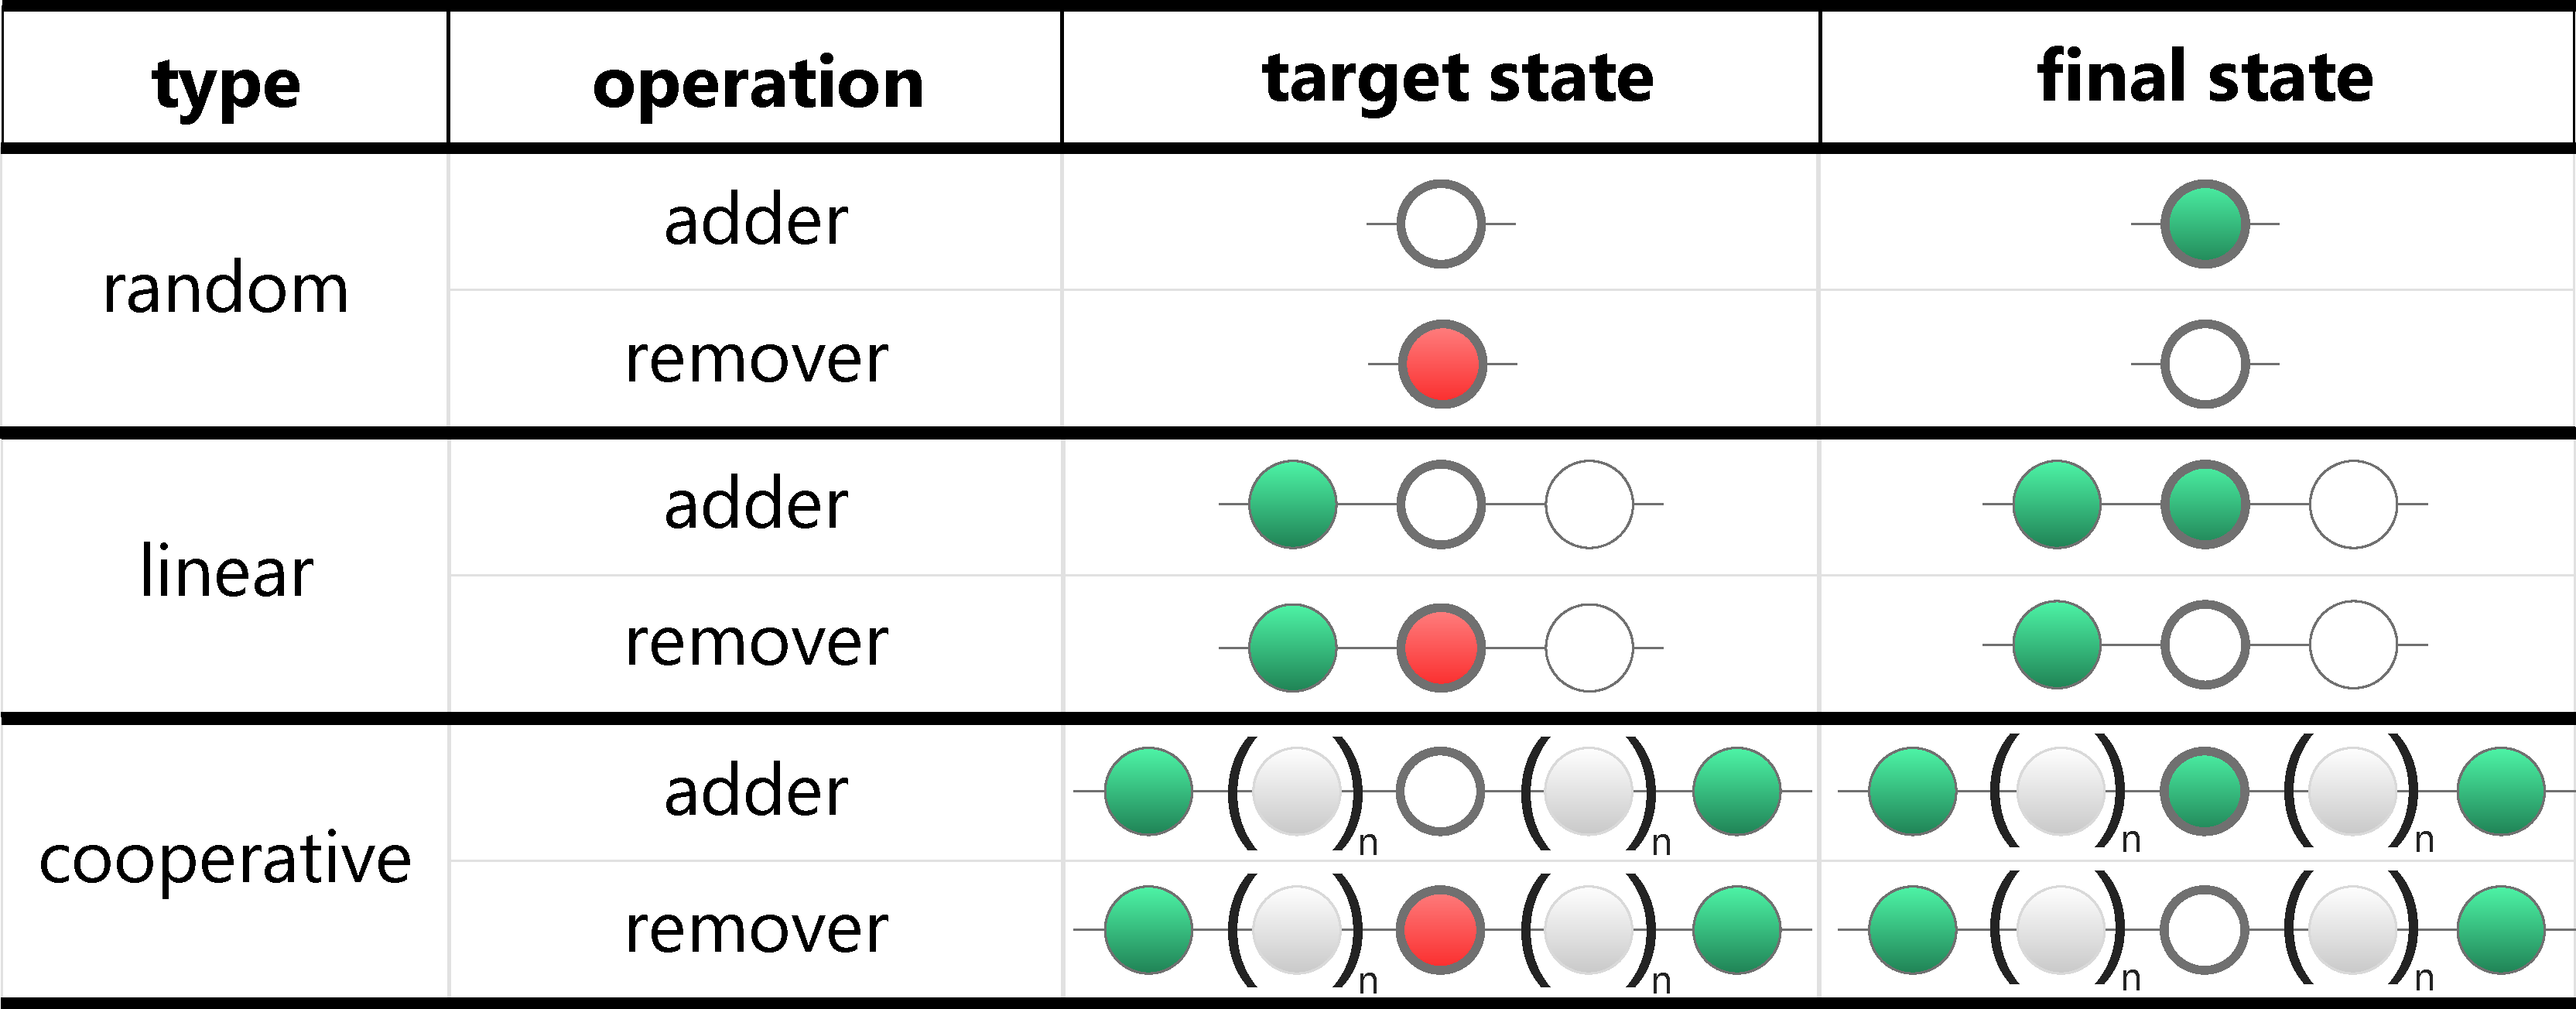
\includegraphics[width=\textwidth]{enzymes/table_newest.pdf}
            \label{img:enzymeTypeSummary}
        \end{table}
        %
        %
    %

    %
    % \section{Summary of simulation parameters}
    %     %

    %     %
    %     \begin{table}[htbp!]
    %         \caption{Summary of the simulation parameters explained in \ref{sec:simulationDetails} sorted by subsections in the 'Results' section.}
    %         \centering
    %         \begin{tabular}{lllllrr}
    %                                     &   &                               & coop?          & cyclic? & \multicolumn{1}{l}{diss?} & \multicolumn{1}{l}{simulation time}  \\
    %             \multicolumn{1}{r}{3.1} & ~ & long                          & no coop        & no      & 100000                    & 5                                    \\
    %             ~                       & ~ & short                         & no coop        & no      & 100000                    & 1                                    \\
    %             \multicolumn{1}{r}{3.2} & ~ & long                          & no coopRem     & no      & 100000                    & 5                                    \\
    %             ~                       & ~ & long                          & w coopRem      & no      & 100000                    & 5                                    \\
    %             ~                       & ~ & short                         & no coopRem     & no      & 100000                    & 1                                    \\
    %             ~                       & ~ & short                         & w coopRem      & no      & 100000                    & 1                                    \\
    %             \multicolumn{1}{r}{3.3} & ~ & long                          & no coopRem     & yes     & 100000                    & 20                                   \\
    %             ~                       & ~ & long                          & w coopRem      & yes     & 100000                    & 20                                   \\
    %             ~                       & ~ & short                         & no coopRem     & yes     & 100000                    & 8                                    \\
    %             ~                       & ~ & short                         & w coopRem      & yes     & 100000                    & 8                                    \\
    %             \multicolumn{1}{r}{3.4} & ~ & long                          & no coopRem     & yes     & 100000                    & 20                                   \\
    %             ~                       & ~ & long                          & no coopRem     & yes     & 100                       & 20                                   \\
    %             ~                       & ~ & short                         & no coopRem     & yes     & 100000                    & 6                                    \\
    %             ~                       & ~ & short                         & no coopRem     & yes     & 100                       & 6                                    \\
    %             \multicolumn{1}{r}{3.5} & ~ & maxReach0 (long)              & no coopRem     & yes     & 100000                    & 20                                   \\
    %             ~                       & ~ & maxReach1                     & no coopRem     & yes     & 100000                    & 20                                   \\
    %             ~                       & ~ & maxReach2                     & no coopRem     & yes     & 100000                    & 20                                   \\
    %             ~                       & ~ & maxReach3                     & no coopRem     & yes     & 100000                    & 20                                   \\
    %             ~                       & ~ & maxReach4                     & no coopRem     & yes     & 100000                    & 20                                   \\
    %             ~                       & ~ & maxReach5                     & no coopRem     & yes     & 100000                    & 20                                   \\
    %             ~                       & ~ & maxReach6                     & no coopRem     & yes     & 100000                    & 20                                   \\
    %             \multicolumn{1}{r}{3.6} & ~ & BivalentBistability
    %             (short) & no coopRem 2 K & yes     & 100000                    & 10                                   \\
    %             ~                       & ~ & FavBivalency (short)          & w coopRem      & yes     & 10000                     & 2                                    \\
    %             ~                       & ~ & FavTotal (short)              & w coopRem      & yes     & 10000                     & 2
    %         \end{tabular}
    %         \label{tab:simulationParametersSummary}
    %     \end{table}
    %     %
    %     %
    %
    %
%	% Run specifications
\chapter{Additional runs}
\label{app:additionalRuns}

\section{Additional runs from section \ref{sec:ResNon-cooperative}}
\label{app:additionalRuns1}

\begin{figure}[htbp!]
    \includeappendixrunplot{appendix_b/31_longRun_nonCyclic_highDiss_0_runHistoryPlot.pdf}
    \includeappendixrunplot{appendix_b/31_longRun_nonCyclic_highDiss_1_runHistoryPlot.pdf}
    \includeappendixrunplot{appendix_b/31_longRun_nonCyclic_highDiss_2_runHistoryPlot.pdf}
    \includeappendixrunplot{appendix_b/31_longRun_nonCyclic_highDiss_3_runHistoryPlot.pdf}
    % \includeappendixrunplot{appendix_b/31_longRun_nonCyclic_highDiss_4_runHistoryPlot.pdf}
    \caption{Runs from 3.1}
\end{figure}

\newpage
\section{Additional runs from section \ref{sec:ResNonCyc}}

\begin{figure}[htbp!]
    \includeappendixrunplot{appendix_b/32_longRun_nonCyclic_highDiss_wCoopRem_0_runHistoryPlot.pdf}
    \includeappendixrunplot{appendix_b/32_longRun_nonCyclic_highDiss_wCoopRem_1_runHistoryPlot.pdf}
    \includeappendixrunplot{appendix_b/32_longRun_nonCyclic_highDiss_wCoopRem_2_runHistoryPlot.pdf}
    \includeappendixrunplot{appendix_b/32_longRun_nonCyclic_highDiss_wCoopRem_3_runHistoryPlot.pdf}
    % \includeappendixrunplot{appendix_b/32_longRun_nonCyclic_highDiss_wCoopRem_4_runHistoryPlot.pdf}
    \caption{Runs from 3.2}
\end{figure}	% Additional runs
% \chapter{Source Code}
    \label{app:SourceCode}
    %

    %
    \section{Used software}
        %
        The source code for the used simulation software, \ed/, can be found at \cite{Herbig2021EpiDynaST}.
        %
    %
    %
    \section{Data and scripts}
        %
        The data generated for this thesis as well as the evaluation scripts can be found at \cite{Krecké2021}.
        %
    %
    %
    \section{Thesis \LaTeX{} code}
        %
        The \LaTeX{} source code for this very thesis can be found at \cite{Krecké2021Thesis}.
        %
    %
    %
%
%




	% chronological list of changes
% \chapter{\latex Source Code}
\label{app:SourceCode}

	% source text of this document

%%%----------------------------------------------------------
\MakeBibliography                        				% references
%%%----------------------------------------------------------

%%% special page for checking print size --------------------
\chapter*{Check Final Print Size}

\begin{center}
{\Large --- Check final print size! ---}

\bigskip

\calibrationbox{100}{50} % width/height of box in mm

\bigskip

{\Large --- Remove this page after printing! ---}

\end{center}



%%%----------------------------------------------------------
\end{document}
%%%----------------------------------------------------------